
 
% ============================================================
\chapter{Weerstandsschatting en aandrijflijn}
\label{ch:holtrop-aandrijflijn}
% ============================================================
 
\section{Weerstandsschatting met de Holtrop-Mennen methode}
\label{sec:holtrop}
 
De totale weerstand van \emph{t~Jansje} in varende conditie is geschat met behulp van de
statistische regressiemethode van Holtrop en Mennen, zoals gepubliceerd in
\cite{Holtrop1984}. Deze methode is geldig voor de varende conditie in zeewater
($\rho = 1025\ \mathrm{kg/m^3}$) bij $15\,^{\circ}\mathrm{C}$, zonder golven.
 
De totale weerstand wordt opgesplitst in de volgende componenten \cite{Holtrop1984}:
 
\begin{equation}
    R_\mathrm{totaal} = R_F(1+k_1) + R_{APP} + R_W + R_B + R_{TR} + R_A
    \label{eq:Rtot}
\end{equation}
 
\noindent waarbij:
\begin{itemize}
    \item $R_F$ de wrijvingsweerstand volgens de ITTC-1957 formulering is,
    \item $(1+k_1)$ de vormfactor van de romp is,
    \item $R_{APP}$ de aanhangselweerstand is (bijv.\ roer, schroefassen),
    \item $R_W$ de golfweerstand is,
    \item $R_B$ de extra weerstand door een boegbulb nabij het wateroppervlak is,
    \item $R_{TR}$ de drukweerstand van een geïmmergeerde spiegel is,
    \item $R_A$ de modelschaalkorrelatieallowance ($C_A$) is, inclusief de
          ruwheidsallowance $\Delta C_F$.
\end{itemize}
 
De wrijvingsweerstand wordt berekend als:
\begin{equation}
    R_F = \frac{1}{2}\,\rho\,V^2\,S\,C_F, \qquad
    C_F = \frac{0.075}{(\log Re - 2)^2}
    \label{eq:RF}
\end{equation}
 
De golfweerstand voor het opererende Froude-getal-gebied ($F_n \leq 0.4$) is:
\begin{equation}
    R_W = c_1\,c_2\,c_5\,\nabla\,\rho\,g \exp\!\bigl[m_1 F_n^d + m_4 \cos(\lambda F_n^{-2})\bigr]
    \label{eq:RW}
\end{equation}
 
\noindent De coëfficiënten $c_1, c_2, c_5, m_1, m_4, \lambda$ zijn uitdrukkingen in de
scheepsparameters $L_{wl}$, $B$, $T$, $C_B$, $C_P$, $C_{wp}$, $C_M$ en $L_{CB}$.
De geldigheidsrange van de methode omvat o.a.:
$0.55 \leq C_P \leq 0.85$, $3.9 \leq L/B \leq 14.9$ en $2.1 \leq B/T \leq 4.0$.
 
\subsection{Scheepsgegevens}
\label{subsec:holtrop-scheepsgegevens}
 
\begin{table}[H]
\centering
\caption{Invoerparameters Holtrop-schatting, \emph{t~Jansje} (varende conditie)}
\label{tab:holtrop_input}
\begin{tabular}{llll}
\toprule
Parameter & Symbool & Waarde & Eenheid \\
\midrule
Lengte waterlijn                            & $L_{wl}$     & 22{,}22 & m        \\
Breedte waterlijn                           & $B$          &  4{,}36 & m        \\
Diepgang achterschip                        & $T_{APP}$    &  1{,}50 & m        \\
Diepgang voorschip                          & $T_{FPP}$    &  1{,}50 & m        \\
Gemiddelde diepgang                         & $T_m$        &  1{,}50 & m        \\
Verdringingsvolume                          & $\nabla$     & 73{,}0  & m$^3$    \\
Hoofdspantcoëfficiënt                       & $C_M$        &  0{,}90 & –        \\
Waterplancoëfficiënt                        & $C_{wp}$     &  0{,}795& –        \\
Blokcoëfficiënt                             & $C_B$        &  0{,}502& –        \\
Prismatische coëfficiënt                    & $C_P$        &  0{,}558& –        \\
Halve instroomhoek                          & $i_E$        & 17      & $^\circ$ \\
LCB-positie (t.o.v.\ $\tfrac{1}{2}L_{wl}$) & $LCB$\%     &  0{,}0  & \%       \\
Spiegeloppervlak                            & $A_T$        & 0       & m$^2$    \\
Transversaal boegbulboppervlak              & $A_{BT}$     & 0       & m$^2$    \\
Sternvormcoëfficiënt                        & $C_{stern}$  & 0       & –        \\
Ruwheidsmaatstaf                            & $k_s$        & 150     & $\mu$m   \\
\bottomrule
\end{tabular}
\end{table}
 
De methode van Holtrop en Mennen is afgeleid via statistische regressie op een proefbestand
van scheepsmodellen. Daardoor gelden geldigheidsranges voor de invoerparameters: buiten deze
ranges kunnen de regressieformules onbetrouwbare uitkomsten geven.
De spreadsheetimplementatie \cite{spreadsheet_holtrop} controleert automatisch acht
geldigheidsvoorwaarden. Tabel~\ref{tab:holtrop_checks} geeft een overzicht.
 
\begin{table}[H]
\centering
\caption{Geldigheidscontroles Holtrop (1984) voor \emph{t~Jansje}}
\label{tab:holtrop_checks}
\begin{tabular}{llccc}
\toprule
Parameter & Voorwaarde & Waarde \emph{t~Jansje} & Geslaagd \\
\midrule
Lengte-breedte verhouding    & $3{,}9 \leq L_{wl}/B \leq 14{,}9$     & 5{,}10     & \cmark \\
Breedte-diepgang verhouding  & $2{,}1 \leq B/T \leq 4{,}0$           & 2{,}91     & \cmark \\
Prismatische coëfficiënt     & $0{,}55 \leq C_P \leq 0{,}85$         & 0{,}558    & \cmark \\
LCB-positie                  & $-5\% \leq LCB\% \leq +5\%$           & 0{,}0\%    & \cmark \\
Halve instroomhoek           & $1^\circ \leq i_E \leq 90^\circ$      & $17^\circ$ & \cmark \\
Hoogte boegbulb boven kiel   & $0 \leq h_B \leq 0{,}6\,T_{FPP}$     & 0          & \cmark \\
Golfweerstandsparameter      & $0{,}01 \leq \lambda \leq 1{,}07$     & 0{,}654    & \cmark \\
Froude-getal (bij 8~kn)      & $F_n \leq 0{,}77$                     & 0{,}279    & \cmark \\
Froude-getal (bij $>$16~kn)  & $F_n \leq 0{,}77$                     & $>$0{,}77  & \times \\
\bottomrule
\end{tabular}
\end{table}
 
Alle checks zijn geslaagd voor de ontwerpsnelheid van 8~knopen. De overschrijding bij snelheden
boven 16~knoop is niet relevant, aangezien \emph{t~Jansje} als historisch binnenvaartschip
nooit op dergelijke snelheden vaart.
 
\subsection{Afgeleide grootheden}
\label{subsec:holtrop-afgeleid}
 
\begin{table}[H]
\centering
\caption{Berekende grootheden op basis van de scheepsgeometrische invoer}
\label{tab:holtrop_derived}
\begin{tabular}{llll}
\toprule
Grootheid & Symbool & Waarde & Eenheid \\
\midrule
Vormfactor            & $(1+k_1)$    & 1{,}2081               & –    \\
Nat oppervlak         & $S$          & 108{,}82               & m$^2$\\
Looplengte            & $L_R$        & 9{,}82                 & m    \\
Correlatie-allowance  & $C_A$        & $7{,}31 \times 10^{-4}$& –    \\
Ruwheidsallowance     & $\Delta C_F$ & $4{,}31 \times 10^{-8}$& –    \\
\bottomrule
\end{tabular}
\end{table}
 
De vormfactor $(1+k_1) = 1{,}208$ geeft aan dat de viskeuze weerstand van de romp ruim 20\%
hoger is dan de vlakke plaatswrijving alleen, wat kenmerkend is voor een relatief vol maar
kort schip met $C_B \approx 0{,}50$.
 
\subsection{Resultaten}
\label{subsec:holtrop-resultaten}
 
Bij de ontwerpsnelheid van 8~knoop ($V = 4{,}116\ \mathrm{m/s}$, $F_n = 0{,}279$) resulteert
de berekening in de weerstandscomponenten van Tabel~\ref{tab:holtrop_results_8kn}.
 
\begin{table}[H]
\centering
\caption{Weerstandscomponenten bij $V = 8\ \mathrm{kn}$}
\label{tab:holtrop_results_8kn}
\begin{tabular}{lrr}
\toprule
Component & Waarde [kN] & Aandeel [\%] \\
\midrule
Wrijvingsweerstand (incl.\ vormfactor) $R_F(1+k_1)$ & 2{,}472 & 55{,}7 \\
Golfweerstand $R_W$                                   & 1{,}276 & 28{,}8 \\
Correlatie-allowance $R_A$                            & 0{,}691 & 15{,}6 \\
Aanhangselweerstand $R_{APP}$                         & 0       &  0{,}0 \\
Spiegelweerstand $R_{TR}$                             & 0       &  0{,}0 \\
Boegbulbweerstand $R_B$                               & 0       &  0{,}0 \\
\midrule
\textbf{Totale weerstand} $R_\mathrm{totaal}$  & \textbf{4{,}439} & \textbf{100{,}0} \\
\midrule
Effectief vermogen EHP & \multicolumn{2}{c}{$18{,}3\ \mathrm{kW}$} \\
\bottomrule
\end{tabular}
\end{table}
 
De wrijvingsweerstand vormt het grootste component (55{,}7\%), in lijn met de verwachtingen voor
een langzaam binnenvaartschip met een laag Froude-getal. Bij 8~knopen is de golfweerstand met
28{,}8\% echter niet langer verwaarloosbaar. Aanhangsels zijn niet gemodelleerd
($R_{APP} = 0$); in de praktijk zal de werkelijke weerstand daardoor licht hoger uitvallen.
 
\begin{table}[H]
\centering
\caption{Weerstand en effectief vermogen als functie van de snelheid}
\label{tab:holtrop_speed_series}
\begin{tabular}{rrrrrrrr}
\toprule
$V$ [kn] & $V$ [m/s] & $F_n$ [–] & $R_F$ [kN] & $R_W$ [kN] & $R_A$ [kN]
         & $R_\mathrm{tot}$ [kN] & EHP [kW] \\
\midrule
5  & 2{,}572 & 0{,}174 & 1{,}036 & 0{,}020 & 0{,}270 & 1{,}326 &  3{,}41 \\
6  & 3{,}087 & 0{,}209 & 1{,}452 & 0{,}123 & 0{,}388 & 1{,}963 &  6{,}06 \\
7  & 3{,}601 & 0{,}244 & 1{,}931 & 0{,}455 & 0{,}529 & 2{,}914 & 10{,}49 \\
\rowcolor{green!15}
8  & 4{,}116 & 0{,}279 & 2{,}472 & 1{,}276 & 0{,}691 & 4{,}439 & 18{,}27 \\
9  & 4{,}630 & 0{,}314 & 3{,}075 & 2{,}351 & 0{,}874 & 6{,}300 & 29{,}17 \\
10 & 5{,}144 & 0{,}348 & 3{,}739 & 4{,}397 & 1{,}079 & 9{,}215 & 47{,}41 \\
\bottomrule
\end{tabular}
\end{table}
 
\subsection{Figuren}
\label{subsec:holtrop-figuren}
 
De resultaten van de Holtrop-schatting zijn weergegeven in vier figuren.
Figuur~\ref{fig:holtrop_rtot} toont de totale weerstand als functie van de snelheid.
Figuur~\ref{fig:holtrop_stacked} geeft de opbouw van de weerstand in drie componenten.
Figuur~\ref{fig:holtrop_ehp} toont het effectief vermogen met markering van de
ontwerpsnelheid. Figuur~\ref{fig:holtrop_pie} geeft de procentuele verdeling bij 8~knoop.
 
% ------------------------------------------------------------------
% Figuur 1: Totale weerstand vs. snelheid
% ------------------------------------------------------------------
\begin{figure}[H]
\centering
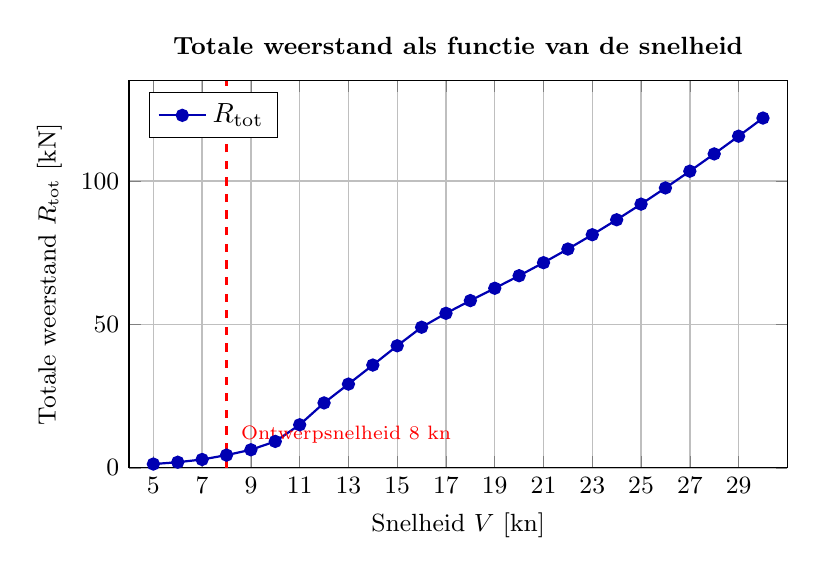
\begin{tikzpicture}
\begin{axis}[
    width  = 0.82\textwidth,
    height = 6.5cm,
    xlabel = {Snelheid $V$ [kn]},
    ylabel = {Totale weerstand $R_\mathrm{tot}$ [kN]},
    title  = {Totale weerstand als functie van de snelheid},
    xmin=4, xmax=31,
    ymin=0, ymax=135,
    xtick={5,7,9,11,13,15,17,19,21,23,25,27,29},
    grid=both,
    grid style={line width=0.3pt, draw=gray!30},
    major grid style={line width=0.5pt, draw=gray!50},
    legend pos=north west,
    tick label style={font=\small},
    label style={font=\small},
    title style={font=\small\bfseries},
]
\addplot[
    color=blue!70!black, thick, mark=*, mark size=2pt,
] coordinates {
    (5,1.3265)(6,1.9634)(7,2.9142)(8,4.4391)(9,6.2999)(10,9.2149)
    (11,15.0227)(12,22.6354)(13,29.1946)(14,35.8332)(15,42.5505)
    (16,49.0182)(17,53.8739)(18,58.2992)(19,62.6043)(20,66.9766)
    (21,71.5172)(22,76.2736)(23,81.2624)(24,86.4828)(25,91.9253)
    (26,97.5756)(27,103.4179)(28,109.4359)(29,115.6139)(30,121.9369)
};
\addlegendentry{$R_\mathrm{tot}$}
\addplot[red, dashed, thick, forget plot]
    coordinates {(8,0)(8,135)};
\node[red, font=\scriptsize, anchor=south west] at (axis cs:8.2,5)
    {Ontwerpsnelheid 8~kn};
\end{axis}
\end{tikzpicture}
\caption{Totale weerstand van \emph{t~Jansje} als functie van de snelheid,
         berekend met de methode van Holtrop~\cite{Holtrop1984}.
         De sterke toename boven 10~knoop is kenmerkend voor het
         golfweerstandshump bij $F_n \approx 0{,}30$--$0{,}35$.}
\label{fig:holtrop_rtot}
\end{figure}
 
% ------------------------------------------------------------------
% Figuur 2: Gestapelde weerstandscomponenten (5-14 kn)
% ------------------------------------------------------------------
\begin{figure}[H]
\centering
\begin{tikzpicture}
\begin{axis}[
    width  = 0.82\textwidth,
    height = 6.5cm,
    xlabel = {Snelheid $V$ [kn]},
    ylabel = {Weerstand [kN]},
    title  = {Weerstandscomponenten (gestapeld, 5--14~kn)},
    xmin=4.5, xmax=14.5,
    ymin=0, ymax=40,
    xtick={5,6,7,8,9,10,11,12,13,14},
    grid=both,
    grid style={line width=0.3pt, draw=gray!30},
    major grid style={line width=0.5pt, draw=gray!50},
    legend pos=north west,
    legend style={font=\small},
    tick label style={font=\small},
    label style={font=\small},
    title style={font=\small\bfseries},
]
\addplot[name path=zero, draw=none, forget plot]
    coordinates {(5,0)(6,0)(7,0)(8,0)(9,0)(10,0)(11,0)(12,0)(13,0)(14,0)};
\addplot[name path=RF, draw=none, forget plot] coordinates {
    (5,1.0363)(6,1.4516)(7,1.9306)(8,2.4722)(9,3.0751)
    (10,3.7386)(11,4.4617)(12,5.2438)(13,6.0842)(14,6.9823)};
\addplot[name path=RFRW, draw=none, forget plot] coordinates {
    (5,1.0567)(6,1.5749)(7,2.3855)(8,3.7485)(9,5.4259)
    (10,8.1359)(11,13.7170)(12,21.0815)(13,27.3710)(14,33.7182)};
\addplot[name path=RFRWRA, draw=none, forget plot] coordinates {
    (5,1.3264)(6,1.9634)(7,2.9142)(8,4.4391)(9,6.2999)
    (10,9.2149)(11,15.0227)(12,22.6353)(13,29.1946)(14,35.8332)};
\addplot[fill=blue!40, fill opacity=0.75, draw=none, area legend]
    fill between[of=RF and zero];
\addlegendentry{$R_F(1{+}k_1)$}
\addplot[fill=red!45, fill opacity=0.75, draw=none, area legend]
    fill between[of=RFRW and RF];
\addlegendentry{$R_W$}
\addplot[fill=yellow!60, fill opacity=0.85, draw=none, area legend]
    fill between[of=RFRWRA and RFRW];
\addlegendentry{$R_A$}
\addplot[blue!70!black, thick, mark=*, mark size=1.8pt, forget plot] coordinates {
    (5,1.0363)(6,1.4516)(7,1.9306)(8,2.4722)(9,3.0751)
    (10,3.7386)(11,4.4617)(12,5.2438)(13,6.0842)(14,6.9823)};
\addplot[red!60!black, thick, forget plot] coordinates {
    (5,1.0567)(6,1.5749)(7,2.3855)(8,3.7485)(9,5.4259)
    (10,8.1359)(11,13.7170)(12,21.0815)(13,27.3710)(14,33.7182)};
\addplot[yellow!60!black, thick, forget plot] coordinates {
    (5,1.3264)(6,1.9634)(7,2.9142)(8,4.4391)(9,6.2999)
    (10,9.2149)(11,15.0227)(12,22.6353)(13,29.1946)(14,35.8332)};
\addplot[red, dashed, thick, forget plot]
    coordinates {(8,0)(8,40)};
\end{axis}
\end{tikzpicture}
\caption{Gestapelde weerstandscomponenten voor \emph{t~Jansje} in het bereik
         5--14~knoop. $R_W$ neemt snel toe boven 7~knoop,
         terwijl $R_F$ bij lage snelheden het grootste aandeel heeft.}
\label{fig:holtrop_stacked}
\end{figure}
 
% ------------------------------------------------------------------
% Figuur 3: EHP vs. snelheid
% ------------------------------------------------------------------
\begin{figure}[H]
\centering
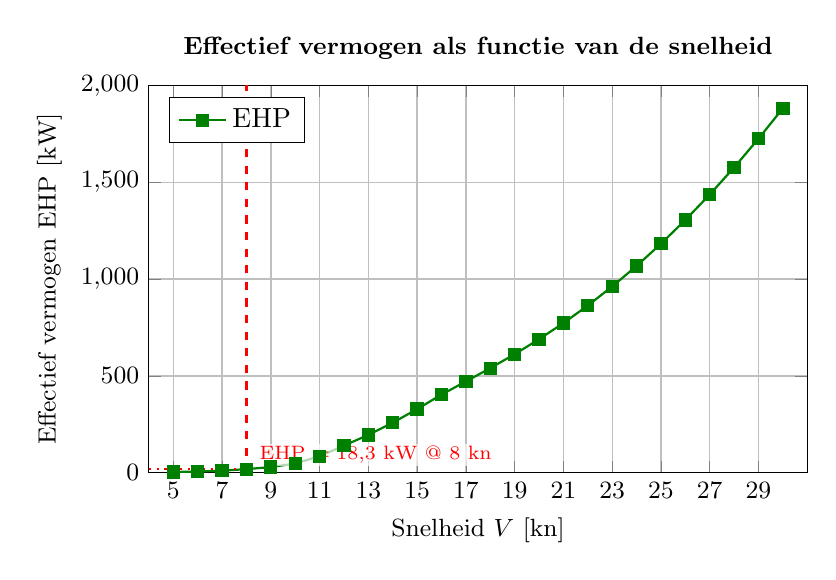
\begin{tikzpicture}
\begin{axis}[
    width  = 0.82\textwidth,
    height = 6.5cm,
    xlabel = {Snelheid $V$ [kn]},
    ylabel = {Effectief vermogen EHP [kW]},
    title  = {Effectief vermogen als functie van de snelheid},
    xmin=4, xmax=31,
    ymin=0, ymax=2000,
    xtick={5,7,9,11,13,15,17,19,21,23,25,27,29},
    grid=both,
    grid style={line width=0.3pt, draw=gray!30},
    major grid style={line width=0.5pt, draw=gray!50},
    legend pos=north west,
    tick label style={font=\small},
    label style={font=\small},
    title style={font=\small\bfseries},
]
\addplot[
    color=green!50!black, thick, mark=square*, mark size=2pt,
] coordinates {
    (5,3.412)(6,6.060)(7,10.494)(8,18.269)(9,29.169)(10,47.406)
    (11,85.012)(12,139.736)(13,195.247)(14,258.078)(15,328.348)
    (16,403.474)(17,471.157)(18,539.850)(19,611.922)(20,689.114)
    (21,772.623)(22,863.247)(23,961.514)(24,1067.773)(25,1182.260)
    (26,1305.127)(27,1436.473)(28,1576.362)(29,1724.829)(30,1881.891)
};
\addlegendentry{EHP}
\addplot[red, dashed, thick, forget plot]
    coordinates {(8,0)(8,2000)};
\addplot[red, dotted, thick, forget plot]
    coordinates {(4,18.269)(8,18.269)};
\node[red, font=\scriptsize, anchor=south west,
      fill=white, fill opacity=0.7, text opacity=1,
      inner sep=1pt] at (axis cs:8.4,30)
    {EHP $= 18{,}3$~kW @ 8~kn};
\end{axis}
\end{tikzpicture}
\caption{Effectief vermogen van \emph{t~Jansje} als functie van de snelheid.
         Bij de ontwerpsnelheid van 8~knoop bedraagt $\mathrm{EHP} = 18{,}3\ \mathrm{kW}$.
         Het daadwerkelijk te installeren vermogen ligt hoger vanwege verliezen
         in de aandrijflijn ($\eta_D$) en operationele marges.}
\label{fig:holtrop_ehp}
\end{figure}
 
% ------------------------------------------------------------------
% Figuur 4: Taartdiagram
% ------------------------------------------------------------------
\begin{figure}[H]
\centering
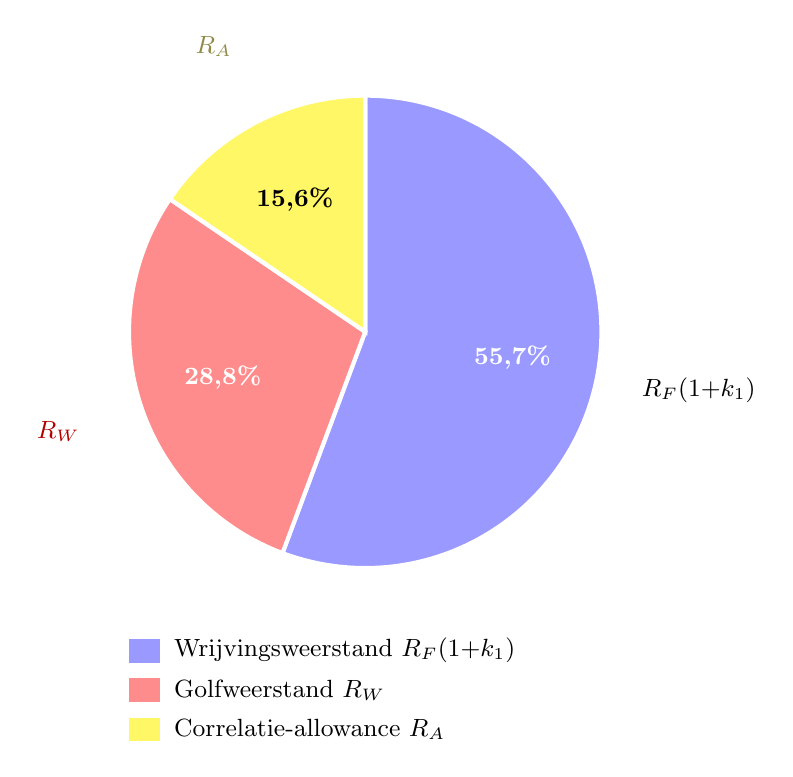
\begin{tikzpicture}
\def\R{3.0cm}
\fill[blue!40, draw=white, line width=1.5pt]
    (0,0) -- ({cos(90)*\R},{sin(90)*\R})
    arc[start angle=90, end angle=-110.5, radius=\R] -- cycle;
\fill[red!45, draw=white, line width=1.5pt]
    (0,0) -- ({cos(-110.5)*\R},{sin(-110.5)*\R})
    arc[start angle=-110.5, end angle=-214.2, radius=\R] -- cycle;
\fill[yellow!60, draw=white, line width=1.5pt]
    (0,0) -- ({cos(-214.2)*\R},{sin(-214.2)*\R})
    arc[start angle=-214.2, end angle=-270, radius=\R] -- cycle;
\node[font=\small\bfseries, white]
    at ({cos(-10)*1.9cm},{sin(-10)*1.9cm}) {55{,}7\%};
\node[font=\small\bfseries, white]
    at ({cos(-162)*1.9cm},{sin(-162)*1.9cm}) {28{,}8\%};
\node[font=\small\bfseries]
    at ({cos(-242)*1.9cm},{sin(-242)*1.9cm}) {15{,}6\%};
\node[font=\small\bfseries, align=left]
    at ({cos(-10)*(\R+1.3cm)},{sin(-10)*(\R+1.3cm)}) {$R_F(1{+}k_1)$};
\node[font=\small\bfseries, text=red!70!black, align=right]
    at ({cos(-162)*(\R+1.1cm)},{sin(-162)*(\R+1.1cm)}) {$R_W$};
\node[font=\small\bfseries, text=yellow!50!black, align=left]
    at ({cos(-242)*(\R+1.1cm)},{sin(-242)*(\R+1.1cm)}) {$R_A$};
\fill[blue!40]  (-3.0,-4.2) rectangle (-2.6,-3.9);
\node[right, font=\small] at (-2.55,-4.05) {Wrijvingsweerstand $R_F(1{+}k_1)$};
\fill[red!45]   (-3.0,-4.7) rectangle (-2.6,-4.4);
\node[right, font=\small] at (-2.55,-4.55) {Golfweerstand $R_W$};
\fill[yellow!60](-3.0,-5.2) rectangle (-2.6,-4.9);
\node[right, font=\small] at (-2.55,-5.05) {Correlatie-allowance $R_A$};
\end{tikzpicture}
\caption{Procentuele verdeling van de weerstandscomponenten bij de
         ontwerpsnelheid van 8~knoop ($R_\mathrm{tot} = 4{,}44\ \mathrm{kN}$).
         De wrijvingsweerstand is dominant (55{,}7\%), terwijl de golfweerstand
         met 28{,}8\% al significant is bij $F_n = 0{,}279$.}
\label{fig:holtrop_pie}
\end{figure}
 
\subsection{Validatie en beperkingen}
\label{subsec:holtrop-validatie}
 
De methode van Holtrop en Mennen is wereldwijd de meest gebruikte statistische methode voor
vroege ontwerpfasen. De geschatte nauwkeurigheid bedraagt doorgaans $\pm5$--$10\%$ voor de
totale weerstand, mits de scheepsparameters binnen de geldigheidsrange vallen
\cite{Holtrop1984, Molland2011}.
 
Voor \emph{t~Jansje} gelden de volgende kanttekeningen:
 
\begin{itemize}
    \item \textbf{Aanhangsels}: Geen roer, schroefas of kielplaat ingevoerd ($R_{APP} = 0$).
          Bij implementatie van een definitief aandrijfconcept dient $R_{APP}$ nader bepaald
          te worden.
    \item \textbf{Ondiepwater-effect}: De methode is ontwikkeld voor diepwater. Het vaargebied
          (Nieuwe Maas, Maassluis) kan ondiepwater-effecten hebben die de weerstand verhogen.
    \item \textbf{Golven en wind}: De berekening geldt voor kalm water. Operationele marges
          voor golfweerstand ($R_{AW}$) en windweerstand ($R_{AA}$) zijn niet meegenomen.
\end{itemize}
 
Ondanks deze beperkingen geeft de Holtrop-schatting een betrouwbare ondergrens voor het
benodigde aandrijfvermogen. Het resultaat – $\mathrm{EHP} = 18{,}3\ \mathrm{kW}$ bij
8~knopen – vormt direct de invoer voor de aandrijflijnanalyse in de volgende sectie.
 
% ============================================================
\section{Doorrekening aandrijflijn}
\label{sec:aandrijflijn}
% ============================================================
 
Met het effectief trekvermogen $P_E$ bekend, kan de volledige aandrijflijn worden doorgerekend
om het minimaal te installeren motorvermogen $P_B$ te bepalen. Deze stap is noodzakelijk
voordat de energiesysteemkeuze en de maximale belading kunnen worden vastgesteld: het
motorvermogen bepaalt namelijk samen met de batterijcapaciteit de maatgevende randvoorwaarden
voor het systeem.
 
\subsection{Propulsion chain}
\label{subsec:propulsion-chain}
 
Figuur~\ref{fig:propulsion-chain} toont de volledige aandrijflijnsketen van scheepsweerstand
tot energiebron, conform het raamwerk van \cite{Molland2011}.
 
% ------------------------------------------------------------------
% TikZ Propulsion Chain diagram
% ------------------------------------------------------------------
\begin{figure}[H]
\centering
\begin{tikzpicture}[
    node distance = 1.1cm and 1.6cm,
    box/.style    = {rectangle, draw=blue!60!black, fill=blue!8,
                     rounded corners=3pt, text width=3.0cm,
                     align=center, font=\small, inner sep=5pt,
                     minimum height=1.2cm},
    eff/.style    = {rectangle, draw=orange!70!black, fill=orange!12,
                     rounded corners=2pt, text width=2.4cm,
                     align=center, font=\scriptsize, inner sep=4pt,
                     minimum height=0.9cm},
    arr/.style    = {-{Stealth[length=6pt]}, thick, blue!60!black},
    effArr/.style = {-{Stealth[length=5pt]}, thick, dashed, orange!70!black},
]
 
% ---- Knooppunten (linker kolom = vermogens) ----
\node[box] (PE)  {Effectief trekvermogen\\[2pt]
                  $P_E = R \cdot V_s$};
 
\node[box, right=of PE] (PT)  {Stuwvermogen\\[2pt]
                                $P_T = T \cdot V_A$};
 
\node[box, right=of PT] (PO)  {Open-water\\propellervermogen\\[2pt]
                                $P_O = 2\pi Q\,n_p$};
 
\node[box, right=of PO] (PP)  {Propellervermogen\\[2pt]
                                $P_P = 2\pi M_p\,n_p$};
 
\node[box, right=of PP] (PS)  {Asvermogen\\[2pt]
                                $P_S = 2\pi M_s\,n_p$};
 
\node[box, right=of PS] (PB)  {Remmend vermogen\\(Brake power)\\[2pt]
                                $P_B = 2\pi M_B\,n_e$};
 
% ---- Efficiëntie-knopen (onder de pijlen) ----
\node[eff, below=0.55cm of PE, xshift=0.8cm] (etaH)
    {Rompdoelm.\\$\eta_H = \dfrac{1-t}{1-w}$};
 
\node[eff, below=0.55cm of PT, xshift=0.8cm] (etaO)
    {Open-water\\$\eta_O = \dfrac{P_T}{P_O}$};
 
\node[eff, below=0.55cm of PO, xshift=0.8cm] (etaR)
    {Rel.\,roterendR.\\$\eta_R = \dfrac{P_O}{P_P}$};
 
\node[eff, below=0.55cm of PP, xshift=0.8cm] (etaS)
    {Asrendement\\$\eta_S = \dfrac{P_P}{P_S}$};
 
\node[eff, below=0.55cm of PS, xshift=0.8cm] (etaGB)
    {Tandwielkast\\$\eta_{GB} = \dfrac{P_S}{k_e P_B}$};
 
% ---- Propulsief rendement (boogpijl bovenaan) ----
\node[eff, above=1.0cm of PO, xshift=1.6cm, text width=3.8cm,
      fill=green!10, draw=green!60!black] (etaD)
    {Propulsief rendement\\
     $\eta_D = \eta_O \cdot \eta_R \cdot \eta_H$};
 
% ---- Pijlen tussen vermogensblokken ----
\draw[arr] (PE) -- (PT);
\draw[arr] (PT) -- (PO);
\draw[arr] (PO) -- (PP);
\draw[arr] (PP) -- (PS);
\draw[arr] (PS) -- (PB);
 
% ---- Efficiëntie-pijlen (dashed, van onder) ----
\draw[effArr] (etaH.north)  -- ++(0, 0.3) -| ($(PE.south)!0.5!(PT.south)$);
\draw[effArr] (etaO.north)  -- ++(0, 0.3) -| ($(PT.south)!0.5!(PO.south)$);
\draw[effArr] (etaR.north)  -- ++(0, 0.3) -| ($(PO.south)!0.5!(PP.south)$);
\draw[effArr] (etaS.north)  -- ++(0, 0.3) -| ($(PP.south)!0.5!(PS.south)$);
\draw[effArr] (etaGB.north) -- ++(0, 0.3) -| ($(PS.south)!0.5!(PB.south)$);
 
% ---- Propulsief rendement: boog van PE naar PP ----
\draw[{Stealth[length=6pt]}-{Stealth[length=6pt]},
      thick, green!60!black, dashed]
    (PE.north) -- ++(0,0.5) -| (etaD.west);
\draw[{Stealth[length=6pt]}-,
      thick, green!60!black, dashed]
    (etaD.east) -- ++(0.3,0) |- (PP.north);
 
% ---- Energiebron rechts van PB ----
\node[box, right=1.4cm of PB, fill=red!8, draw=red!60!black,
      text width=2.2cm] (Qf)
    {Warmte-input\\$\dot{Q}_f$\\(Energiebron)};
\node[eff, below=0.55cm of PB, xshift=0.8cm,
      fill=red!10, draw=red!60!black, text width=2.4cm] (etaE)
    {Motorrendement\\$\eta_e = P_B/\dot{Q}_f$};
\draw[arr, red!60!black] (PB) -- (Qf);
\draw[effArr, red!70!black] (etaE.north) -- ++(0,0.3) -|
    ($(PB.south east)!0.5!(Qf.south west)$);
 
\end{tikzpicture}
\caption{Aandrijflijnsketen van \emph{t~Jansje}: van effectief trekvermogen $P_E$
         (scheepsweerstand maal snelheid) via de propulsieve verliezen naar het
         remmend vermogen $P_B$ (motoruitlaatas). Oranje blokken geven de
         efficiënties aan die de overgang tussen opeenvolgende
         vermogens beschrijven. Het groene blok toont het propulsief rendement
         $\eta_D = \eta_H \cdot \eta_O \cdot \eta_R$ dat de keten
         van $P_E$ naar $P_P$ in één stap samenvat.
         Gebaseerd op \cite{Molland2011}.}
\label{fig:propulsion-chain}
\end{figure}
 
\subsection{Keuze en onderbouwing van de rendementwaarden}
\label{subsec:rendementen}
 
Voor de keuze van de rendementwaarden is onderscheid gemaakt tussen twee scenario's:
\textbf{scenario~A} (bestaande schroef met tandwielkast, conservatief referentiescenario)
en \textbf{scenario~B} (elektrische direct-drive motor zonder tandwielkast, het beoogde
verduurzamingsconcept). Beide scenario's worden in Tabel~\ref{tab:rendementen} weergegeven.
 
\begin{table}[H]
    \centering
    \caption{Rendementwaarden aandrijflijn \emph{t~Jansje} – twee scenario's met onderbouwing}
    \label{tab:rendementen}
    \begin{tabular}{p{3.2cm} l p{1.2cm} p{1.2cm} p{6.0cm}}
        \toprule
        Rendement & Symbool & Sc.\,A & Sc.\,B & Onderbouwing \\
        \midrule
        Rompdoelmatigheid
            & $\eta_H$
            & 1{,}05
            & 1{,}05
            & Voor volle enkelscharige rompen geldt $t < w$, zodat
              $\eta_H = (1-t)/(1-w) > 1$.
              Typisch $w \approx 0{,}20$ en $t \approx 0{,}15$ voor een
              beurtvaarder op binnenwateren \cite{Molland2011}. \\[6pt]
        Open-water rendement
            & $\eta_O$
            & 0{,}58
            & 0{,}60
            & Scenario~A: bestaande schroef geoptimaliseerd voor diesel
              ($n_p$ hoog, kleine diameter). Scenario~B: bij een elektrische
              direct-drive motor kan de schroef worden herontworpen voor een
              lager toerental en grotere diameter, wat $\eta_O$ merkbaar
              verbetert tot 0{,}60--0{,}62 \cite{Molland2011, Schneekluth1998}. \\[6pt]
        Relatief-roterendrendement
            & $\eta_R$
            & 1{,}03
            & 1{,}03
            & Voor een enkelscharig schip achter een symmetrische achtersteven
              is $\eta_R$ doorgaans licht groter dan~1 (typisch 1{,}02--1{,}05).
              De niet-uniforme instroom verbetert de propellerprestatie ten
              opzichte van vrij water \cite{Molland2011}. \\[6pt]
        Asrendement
            & $\eta_S$
            & 0{,}98
            & 0{,}99
            & Scenario~B: bij een directe koppeling motor–as vervalt de
              tussenliggende asleiding; de korte as heeft minimale
              lagerverliezen ($\eta_S \approx 0{,}99$). \\[6pt]
        Tandwielkastrendement
            & $\eta_{GB}$
            & 0{,}97
            & –
            & Scenario~A: enkelvoudige tandwielkast, typisch 0{,}97--0{,}99
              \cite{Molland2011}. Scenario~B: de tandwielkast vervalt volledig
              bij een variabel-toerentaal elektromotor (VFD), waarvoor in
              de plaats het motorrendement $\eta_\mathrm{em} = 0{,}95$ en het
              omrichterrendement $\eta_\mathrm{inv} = 0{,}97$ worden
              meegenomen. \\[6pt]
        Elektromotor + omrichter
            & $\eta_\mathrm{em} \cdot \eta_\mathrm{inv}$
            & –
            & 0{,}922
            & Moderne PMSM-elektromotoren bereiken $\eta_\mathrm{em} \geq 0{,}95$;
              gecombineerd met een VFD-omrichter ($\eta_\mathrm{inv} = 0{,}97$)
              levert dit $0{,}95 \times 0{,}97 = 0{,}922$, gunstiger dan een
              tandwielkast maar inclusief omrichterverliezen. \\
        \bottomrule
    \end{tabular}
\end{table}
 
\subsection{Stap-voor-stap doorrekening}
\label{subsec:aandrijflijn-berekening}
 
De doorrekening volgt de keten van Figuur~\ref{fig:propulsion-chain} en wordt hier uitgewerkt
voor het beoogde elektrische concept (scenario~B). Ter vergelijking zijn de resultaten voor
scenario~A in Tabel~\ref{tab:aandrijflijn-overzicht} meegenomen.
 
\subsubsection*{Stap 1 – Effectief trekvermogen $P_E$}
 
Het effectief trekvermogen is direct uit de Holtrop-schatting
(Tabel~\ref{tab:holtrop_results_8kn}) verkregen:
 
\begin{equation}
    P_E = R_\mathrm{totaal} \times V
        = 4{,}439\ \mathrm{kN} \times 4{,}116\ \mathrm{m/s}
        = \mathbf{18{,}3}\ \mathbf{kW}.
    \label{eq:PE}
\end{equation}
 
\subsubsection*{Stap 2 – Propulsief rendement $\eta_D$ (scenario~B)}
 
\begin{equation}
    \eta_D = \eta_H \cdot \eta_O \cdot \eta_R
           = 1{,}05 \times 0{,}60 \times 1{,}03
           = \mathbf{0{,}649}.
    \label{eq:etaD}
\end{equation}
 
\subsubsection*{Stap 3 – Propellervermogen $P_P$}
 
\begin{equation}
    P_P = \frac{P_E}{\eta_D}
        = \frac{18{,}3}{0{,}649}
        = \mathbf{28{,}2}\ \mathbf{kW}.
    \label{eq:PP}
\end{equation}
 
\subsubsection*{Stap 4 – Asvermogen $P_S$}
 
\begin{equation}
    P_S = \frac{P_P}{\eta_S}
        = \frac{28{,}2}{0{,}99}
        = \mathbf{28{,}5}\ \mathbf{kW}.
    \label{eq:PS}
\end{equation}
 
\subsubsection*{Stap 5 – Remmend vermogen $P_B$ (aan de motoras)}
 
Bij scenario~B vervangt de combinatie elektromotor + omrichter de tandwielkast:
 
\begin{equation}
    P_B = \frac{P_S}{\eta_\mathrm{em} \cdot \eta_\mathrm{inv}}
        = \frac{28{,}5}{0{,}922}
        = \mathbf{30{,}9}\ \mathbf{kW}.
    \label{eq:PB}
\end{equation}
 
\subsubsection*{Stap 6 – Minimaal te installeren motorvermogen $P_{B,\mathrm{inst}}$}
 
Het berekende $P_B = 30{,}9$~kW is een ondergrens in kalm water. Een operationele marge
van 20\% compenseert voor aanhangsels ($+3$--$5\%$), ondiepwatereffecten op de Nieuwe
Maas ($+2$--$4\%$) en een reserve voor manoeuvreren en tegenwind ($+10$--$15\%$):
 
\begin{equation}
    P_{B,\mathrm{inst}} = P_B \times (1 + f_\mathrm{marge})
                        = 30{,}9 \times 1{,}20
                        = \mathbf{37{,}1}\ \mathbf{kW}
                        \approx \mathbf{37}\ \mathbf{kW}.
    \label{eq:PB-inst}
\end{equation}
 
\subsection{Overzicht aandrijflijn}
\label{subsec:aandrijflijn-overzicht}
 
\begin{table}[H]
    \centering
    \caption{Samenvatting aandrijflijn \emph{t~Jansje} bij $V = 8$~kn – twee scenario's}
    \label{tab:aandrijflijn-overzicht}
    \begin{tabular}{llrrrl}
        \toprule
        Stap & Grootheid & Sc.\,A [kW] & Sc.\,B [kW] & Rendement (B) & Toelichting \\
        \midrule
        1 & $P_E$ (Holtrop)            & 18{,}3 & 18{,}3 & –             & Kalm water, 8~kn \\
        2 & $\eta_D$                   & 0{,}628 & 0{,}649 & –            & $\eta_H \cdot \eta_O \cdot \eta_R$ \\
        3 & $P_P$ (propeller)          & 29{,}1 & 28{,}2 & $0{,}649$     & $P_E/\eta_D$ \\
        4 & $P_S$ (as)                 & 29{,}7 & 28{,}5 & $0{,}99$      & $P_P/\eta_S$ \\
        5 & $P_B$ (motor)              & 30{,}6 & 30{,}9 & $0{,}922$     & $P_S/(\eta_\mathrm{em}\eta_\mathrm{inv})$ \\
        6 & $P_{B,\mathrm{inst}}$      & \textbf{37} & \textbf{37} & – & Incl.\ 20\% marge \\
        \midrule
        \multicolumn{2}{l}{$\eta_\mathrm{totaal} = P_E/P_B$}
          & 0{,}599 & 0{,}592 & \multicolumn{2}{l}{Beide $\approx 60\%$} \\
        \bottomrule
    \end{tabular}
\end{table}
 
Opmerkelijk is dat ondanks de hogere $\eta_O$ in scenario~B het totaalrendement nagenoeg
gelijk blijft aan scenario~A. De winst bij de schroef wordt gecompenseerd door de omrichter-
verliezen. Het voordeel van scenario~B zit dan ook niet primair in een hoger rendement, maar
in de wegvallende onderhoudskosten van de tandwielkast, de betere regelbaarheid van het
toerental en de mogelijkheid tot regeneratief remmen bij het aanmeren.
 
\subsection{Conclusie aandrijflijn}
\label{subsec:aandrijflijn-conclusie}
 
Op basis van de Holtrop-Mennen schatting ($P_E = 18{,}3$~kW bij 8~kn) en realistische
rendementwaarden voor een elektrisch verduurzaamd beurtschip bedraagt het minimaal benodigde
geïnstalleerde motorvermogen $P_{B,\mathrm{inst}} \approx \mathbf{37\ kW}$, ongeacht het
gekozen scenario. Dit is aanmerkelijk lager dan het huidig geïnstalleerde dieselvermogen van
$\approx 82$~kW (110~pk), wat aantoont dat verduurzaming technisch ruim haalbaar is qua
vermogensbehoefte. De aandrijflijnresultaten vormen, samen met de energiebalans uit
Hoofdstuk~\ref{ch:operationeel-profiel}, de directe invoer voor de stabiliteits- en
beladingsberekening in het volgende hoofdstuk.
 